%!TEX root = ../../../adrien_gomar_phd.tex


\begin{figure}
  \centering
  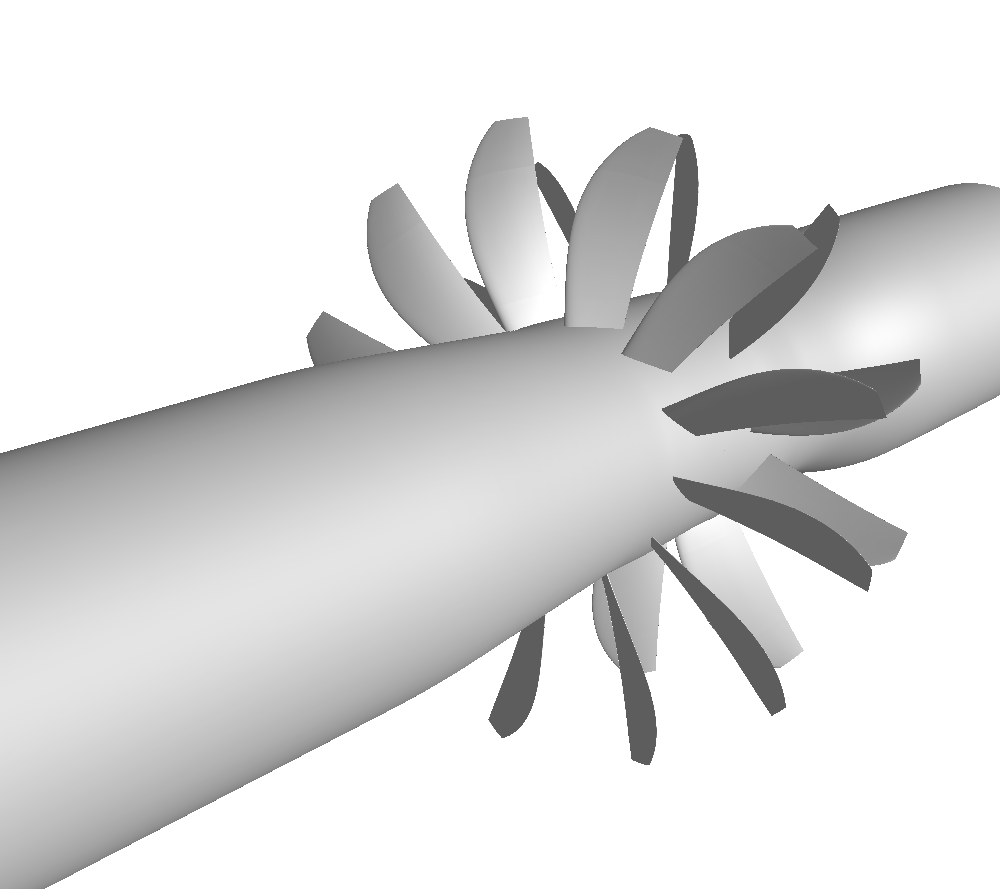
\includegraphics[width=.3\textwidth]{DREAM_LS_wall.png}
  \caption{Low-speed isolated contra-rotating open rotor geometry.}
  \label{fig:dream_ls_wall}
\end{figure}

The studied configuration is a pusher contra-rotating open rotor
that comes from the know-how of SAFRAN-Snecma. Therefore,
neither true geometry nor the absolute values of the variables
will be shown.
The geometry is shown in Fig.~\ref{fig:dream_ls_wall} for the
Low-speed (LS) flight condition, representative of the take-off. 
The simulated configuration does not include the spinner as the
experimental setup does not include this part of the geometry.
Sadly, the experimental results were not available for comparison
at the time this PhD thesis has been written.

\begin{table}
  \ra{1.3} \centering
  \begin{tabular}{cccc}
    \toprule
    $M_0$ & $|\Omega|$ & $J$ & $M_{tip}$ \\
    \midrule
    $0.2$ & $5739$ tr.min\textsuperscript{-1} & 1.06 & 0.63 \\
    \bottomrule
  \end{tabular}
  \caption{Low-speed isolated contra-rotating open rotor flight condition parameters.}
  \label{tab:dream_ls_flight_condition}
\end{table} 
Table~\ref{tab:dream_ls_flight_condition} recalls the main
parameters of the case: the inflow Mach number $M_0$,
the absolute value of the rotation speed of both rotors $|\Omega|$,
the advance ratio $J$ (whose definition is given in Chap.~\ref{cha:cror})
and the Mach number at the tip of
the blade based on the inflow velocity and the advance ratio:
\begin{equation}
	M_{tip} = M_0 \sqrt{1 + \left(\frac{\pi}{J} \right)^2}
\end{equation}
This equation is a simple transcription of the velocity triangle
applied to the infinite velocity and to the rotation speed perceived
at the front blade tip:
\begin{equation}
    M_{tip} = M_0 \sqrt{1 + \left(\frac{\pi}{J}\right)^2} = 
    \frac{V_0}{\sqrt{\gamma R T_0}} \sqrt{1 + \left(\frac{
    	\cancel{\pi} \cdot \Omega D}{
    	2 \cancel{\pi} \cdot V_0}\right)^2} =
    \sqrt{\frac{V_0^2 + (\Omega R)^2}{\gamma R T_0}}
    \label{eq:m_tip_explained}
\end{equation}

The inflow Mach number $M_0$ is in the incompressible range.
Thus, for computations to converge, a preconditionner might be
needed. Hopefully, the rotation of the rotors accelerates the fluid
and the tip Mach number is high enough to not use any preconditionning.
However, let us bare in mind that this range of Mach number might
be tedious for a compressible flow solver.
The advance ratio $J$ is around~1 which is a classical value for
low-speed flight conditions. Note that the rotation speed is large
for a CROR which is more likely to be around 500~tr.min\textsuperscript{-1}.
In fact, a full-scale CROR diameter is around 5~meters. With this rotation speed,
this would lead to a tip Mach number greater than~4. This high rotation speed is 
therefore here to compensated for the small radius of the blades which is~33~cm
while preserving the similarity coefficients for experiment to be reliable.
